\documentclass{beamer}

\usepackage{geometry} % Pour passer au format A4
\usepackage{graphicx} % Required for including pictures
\usepackage{float} % 

\usepackage{amsmath,amsfonts,amssymb,amsthm}
\usepackage[T1]{fontenc} 
\usepackage[english,francais]{babel}
\usepackage[utf8]{inputenc}
\usepackage{lmodern}
\usepackage{eurosym} % signe Euros
\usepackage{verbatim}

\usetheme{Warsaw}

\title{Fonctions}
\author{$2^{nd}1$}

\begin{document}

\frame{\titlepage}

\section{Représentation d'une fonction}

\begin{frame}
  \frametitle{I - Représentation d'une fonction}

  \begin{block}{1 - Tableau de valeurs}	

    \begin{center}
      \begin{tabular}{| l || c | c | c | c | c |}
        \hline			
        x    &  1 & 2 & 3 & 4 & 5\\
        \hline  
        f(x) & -3 & 0 & 3 & 6 & 9\\
        \hline  
      \end{tabular}
    \end{center}

  \end{block}

  \begin{block}{2 - Représentation graphique}
    \begin{figure}[H]
      \centering
      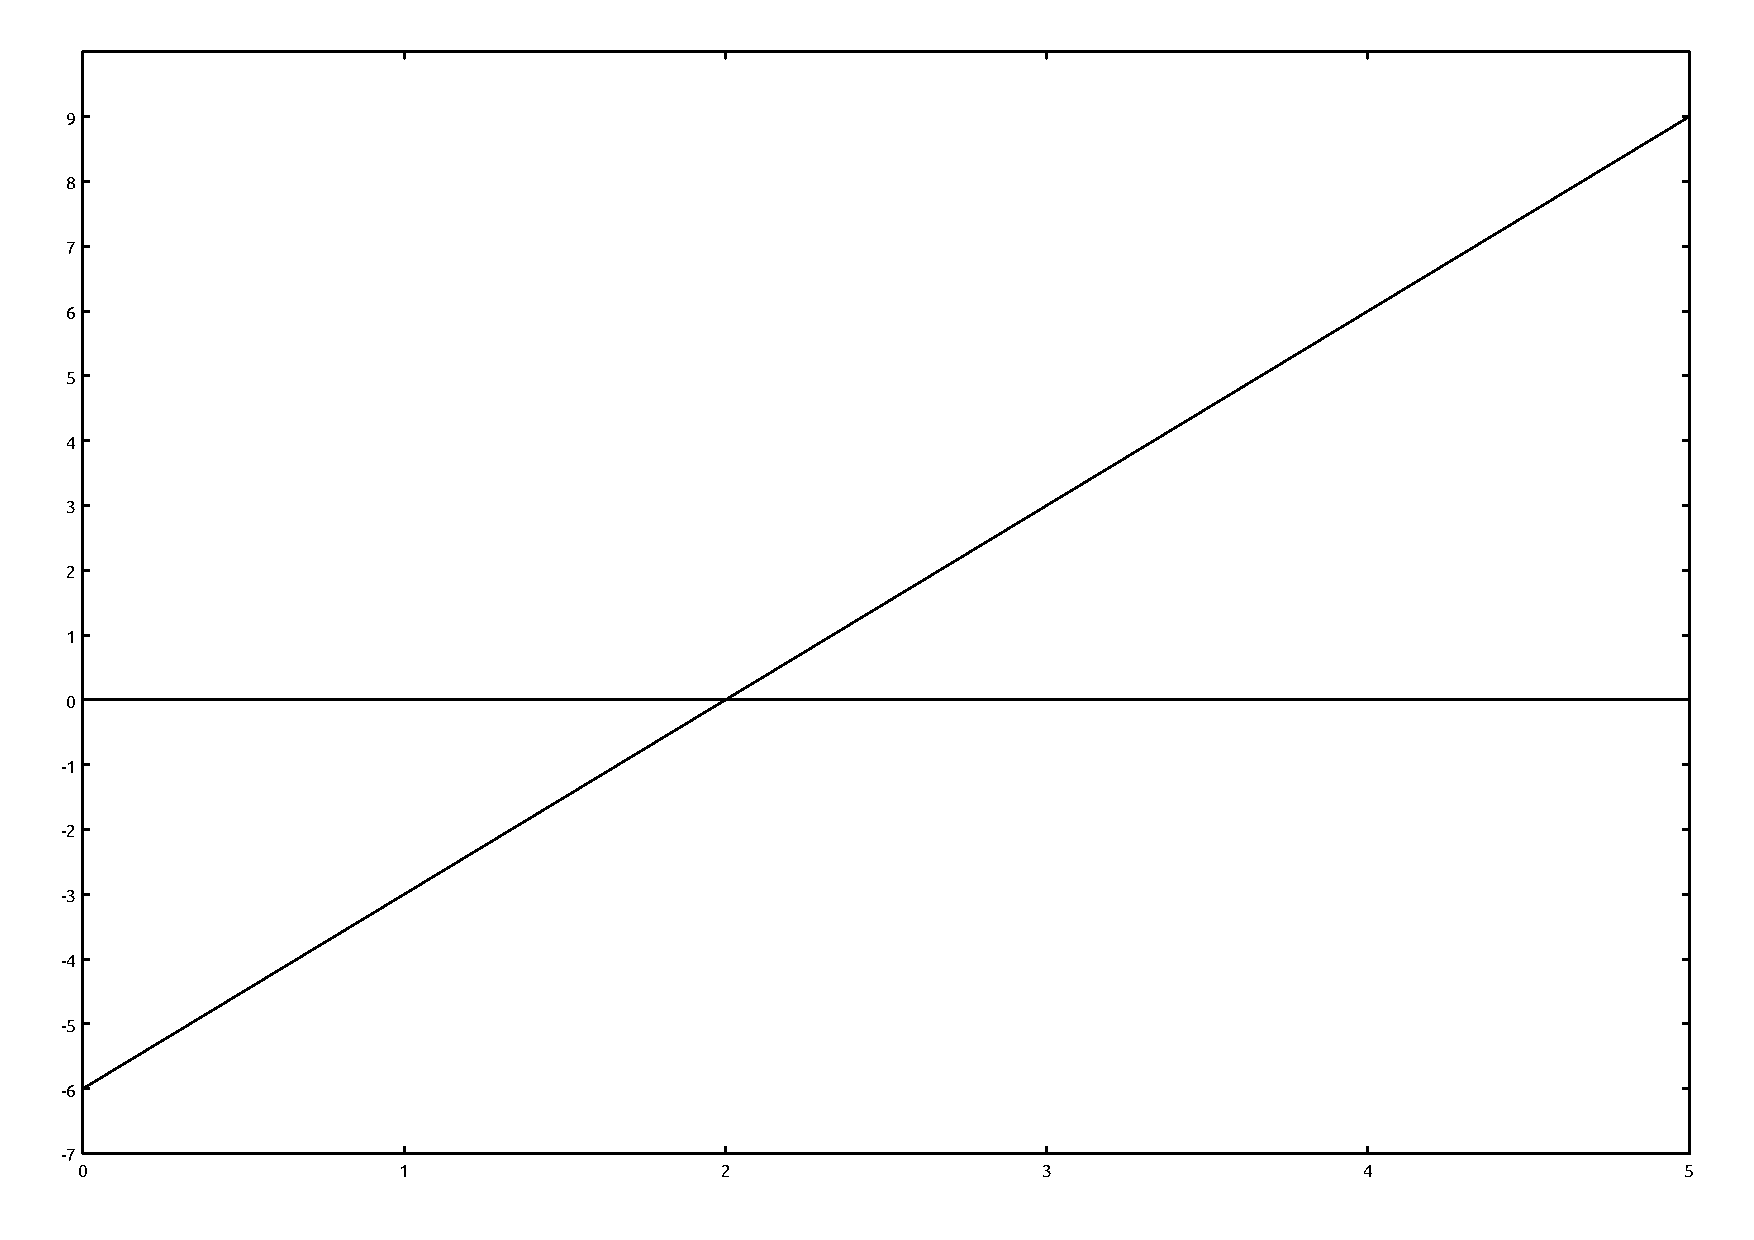
\includegraphics[width=0.6\linewidth]{sources/cours/droite.pdf}
    \end{figure}
  \end{block}

\end{frame}

\begin{frame}
  \frametitle{I - Représentation d'une fonction}

  \begin{block}{3 - Algorithme / Programme de calcul}	
    \begin{itemize}
    \item Choisir x;\\
    \item Soustraire 2;\\
    \item Multiplier le résultat par 3;\\
    \item Affichier le résultat;
    \end{itemize}
  \end{block}

  \begin{alertblock}{4 - Expression littérale}
    $f(x) = (x - 2) \times 3 $
  \end{alertblock}

\end{frame}

\section{Vocabulaire}

\begin{frame}
  \frametitle{II - Vocabulaire}

  \begin{block}{}	
    On appelle $f$ la fonction qui a tout $x$ associe la valeur $f(x)$.
  \end{block}

  \begin{alertblock}{1 - Images}
    $y = f(x)$ est l'image de $x$ par la fonction $f$.
    \begin{itemize}
    \item -3 est l'image de 1 par la fonction $f$.\\
    \item 6 est l'image de 4 par la fonction $f$.
    \end{itemize}
  \end{alertblock}

  \begin{alertblock}{2 - Antécédents}
    $x$ est l'antécédent de $y$ par la fonction $f$.
    \begin{itemize}
    \item 2 est l'antécédent de 0 par la fonction $f$.\\
    \item 5 est l'antécédent de 9 par la fonction $f$.
    \end{itemize}
  \end{alertblock}

\end{frame}


\begin{frame}
  \frametitle{II - Vocabulaire}

  \begin{exampleblock}{Remarques}
    \begin{itemize}
    \item Il peut avoir plusieurs antécédents.
    \item Il y a toujours qu'une seule et unique image.
    \end{itemize}
  \end{exampleblock}

  \begin{figure}[H]
    \centering
    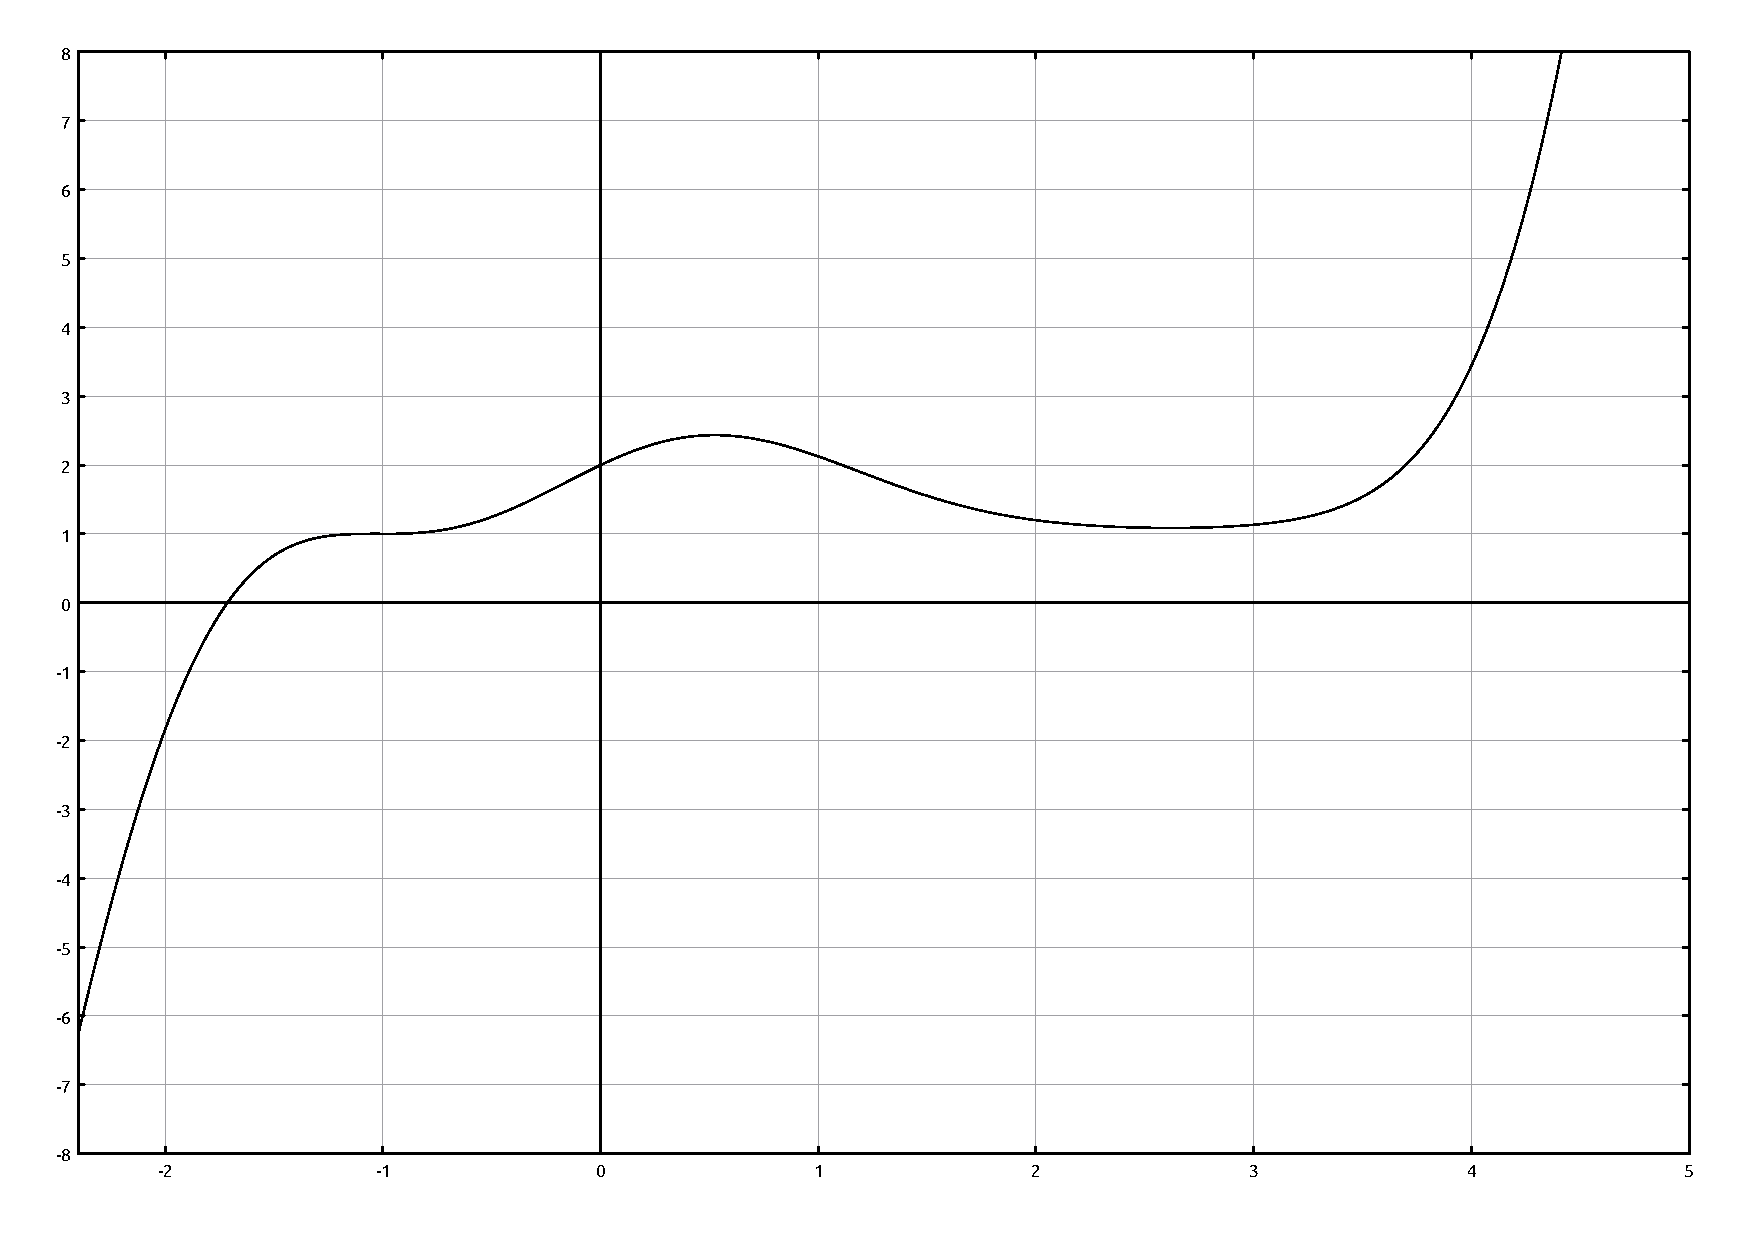
\includegraphics[width=0.56\linewidth]{sources/cours/courbe.pdf}
    \caption{$0$, $1$ et $3.7$ sont les antécédents de $2$ par la fonction $f$.}
  \end{figure}

\end{frame}

\section{ Domaine de définition}
\subsection{Intervalles}

\begin{frame}
  \frametitle{III - Domaine de définition}

  \begin{block}{}	
    Parfois certaines fonctions ne sont définies que pour certaines valeurs de $x$. On utilise la notion d'intervalle.
  \end{block}

  \begin{columns}[t]
    \begin{column}{6cm}

      \begin{block}{1 - Intervalles}

        \begin{columns}[t]
          \begin{column}{3cm}
            \begin{eqnarray*}
    x \in [-1      ; 5     ]\\
    x \in ] 0.5    ; 8     ]\\
    x \in ] 0      ; 9     [\\
    x \in [-5.2    ; -2    [\\
    x \in ]-\infty ; 7     ]\\
    x \in ] 2.5    ; \infty[\\
  \end{eqnarray*}


          \end{column}
          \begin{column}{3cm}  
  \begin{eqnarray*}
    -1   \leq x \leq  5\\
    0.5  <    x \leq  8\\
    0    <    x <     9\\
    -5.2 \leq x \leq -2\\
    x    \leq 7\\
    x    > 2.5\\
  \end{eqnarray*}
          \end{column}
        \end{columns} 

      \end{block}
    \end{column}
    \begin{column}{4cm}  
      \begin{figure}[H]
        \centering
        \includegraphics[width=\linewidth]{sources/cours/intervalles.pdf}
      \end{figure}
    \end{column}
  \end{columns} 

\end{frame}

\subsection{Opérations sur les intervalles}

\begin{frame}
  \frametitle{III - Domaine de définition}

  \begin{block}{2 - Opérations sur les intervalles}
  \end{block}

  \begin{exampleblock}{a) Union}
    Appartenir à l'union de deux intervalles est possible si l'on appartient à l'un OU l'autre des intervalles.
  \end{exampleblock}

  \begin{figure}[H]
    \centering
    \includegraphics[width=0.6\linewidth]{sources/cours/union.pdf}
    \caption{}
  \end{figure}

\end{frame}



\begin{frame}
  \frametitle{III - Domaine de définition}

  \begin{exampleblock}{b) Intersection}
Appartenir à l'intersection de deux intervalles est possible si l'on appartient à l'un ET l'autre des intervalles, (au deux intervalles en même temps).
  \end{exampleblock}

  \begin{figure}[H]
    \centering
    \includegraphics[width=0.6\linewidth]{sources/cours/intersection.pdf}
    \caption{}
  \end{figure}

\end{frame}

\end{document}
